% !TeX spellcheck = en_US
% !TeX root = ./0_article.tex

\section{Modeling and simulating BBI}
\IEEEPARstart{S}{imulating} a fault injection method behavior is an important part in understanding its mechanisms.
Whether it is EMFI, LFI or BBI, it allows to predict and understand the underlying phenomena at work to set up reliable experiments.
In this paper, we are focusing solely on BBI.

Ideally, we would want to directly observe signals inside integrated circuits, allowing for fine measurements of power supply voltages, logic levels and power current not to cite every physical quantity.
However, embedding sensors into an already existing IC is not possible, and doing so on future IC is costly and takes time to fully implement.
In addition to this, we do not have any guarantee that these sensors will not be disturbed too much by the fault injection.
Therefore, we have decided to take the following approach:
\begin{center}
	Simulation \textrightarrow\ Conclusions \textrightarrow\ Verification
\end{center}

By doing so, we have freed ourselves from hardware limitations.
However, other limitations remains.
Indeed, modern ICs, even the smallest, embed millions of transistors, and with current technologies, it is impossible to evaluate with simulations entire circuits at a transistor level.
Therefore, to tackle these limitations, we decided to adopt an hybrid approach, combining transistor-less models and local logic gates simulations.
This approach is a compromise between accuracy and computational cost/time, and allows simulating relatively big circuits under BBI disturbances
Overall, it is similar to what has been done for EMFI in \cite{mathieuEMFI}.
The resulting simulation flow is divided in three consecutive steps:
\begin{itemize}
	\item The simulation of an IC under BBI using a transistor-less model, allowing for a purely electrical analysis;
	\item The extraction of significant disturbed signals from the previous simulation;
	\item The simulation of functional logic gates under BBI thanks to the previously extracted signals.
\end{itemize}

\subsection{An hybrid simulation flow: building the models}
	Building the correct models for the simulation flow pass through multiple steps.
	As the goal of the hybrid flow is to reduce the computational power required to evaluate an IC, it is still important to maintain a certain accuracy concerning the IC physical structure.
	To do so, the models are designed around actual IC implementations.
	The main building blocks of the models are the power supply network, the standard-cells, and the substrate structure.
	In this work, we are only focusing on bulk substrates: specifically dual-well and triple-well substrates.

	\subsubsection{Power supply rails and standard-cell segments}
	% !TeX spellcheck = en_US
% !TeX root = ./0_article.tex
% LABEL AFTER CAPTION WESH GEOFFREY !!
\begin{figure}[h]
	\centering
	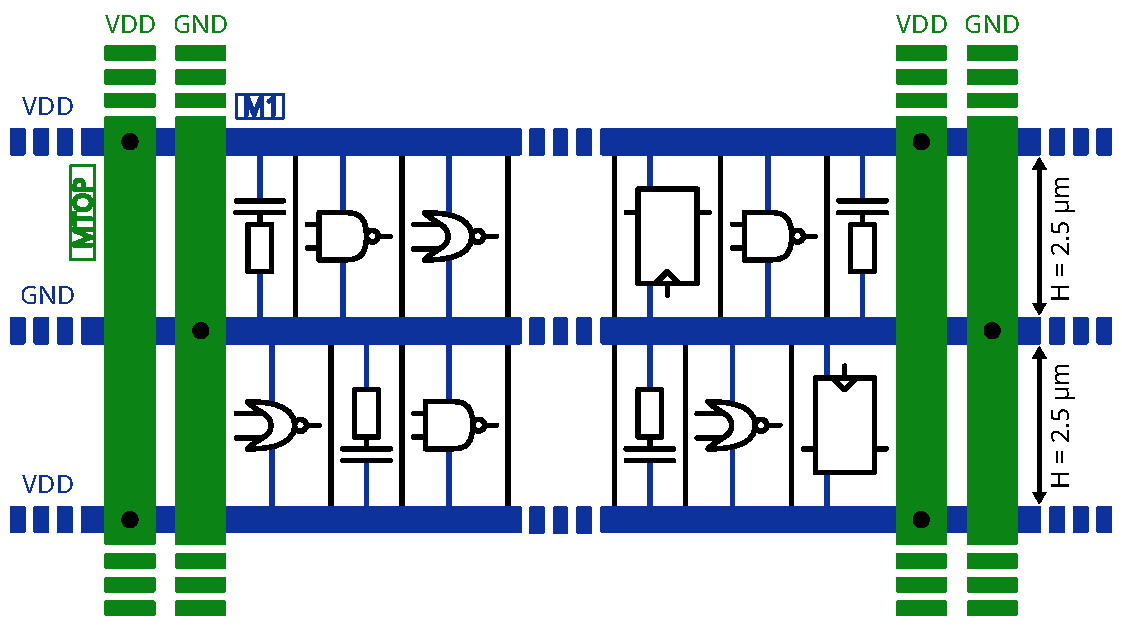
\includegraphics[width=0.49\textwidth]{./figures/psu_std_cell.pdf}
	\caption{A Standard-Cell Segment and its power delivery network.}
	\label{fig_alim_std}
\end{figure}

	The power distribution inside an IC is typically made with a grid-like structure, composed of metal wires stacked on top of each other on planes.
	In each layer, the metal wires are equally spaced and have a dedicated width, which becomes thinner the deeper they are.
	The lowest layer brings the power directly to the transistors.
	Fig. \ref{fig_alim_std} presents a common power delivery network, designed with two metal levels for simplicity.

	Within the metal lines are located standard-cell segments (SCS), composed of decoupling, logic and sequential elements, and are pre-characterized by foundries and categorized depending on their performance (mainly but not exclusively power consumption and speed).
	As illustrated in Fig. \ref{fig_alim_std}, SCS have a constant height, in our case of 2.5 \textmu m, and a variable width depending on how much logic gates each one of them embed.

	\subsubsection{The substrate}
	% !TeX spellcheck = en_US
% !TeX root = ./0_article.tex

\begin{figure}[h]
	\centering
	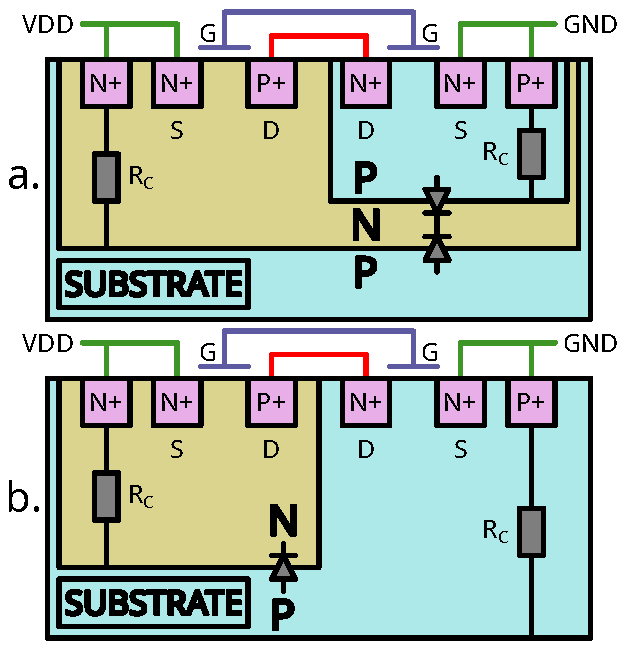
\includegraphics[width=0.35\textwidth]{./figures/substrate_2.pdf}
	\caption{Triple-well (a) and Dual-well (b) inverter cross-sectional view.}
	\label{fig_sub}
\end{figure}

	Because BBI can be performed thanks to the silicon substrate as the main physical environment transferring energy from a generator to an IC, it is fundamental to elaborate a proper substrate model to precisely represent the various involved phenomena.
	As stated previously, our work focuses on bulk substrates, and in most cases, the substrate silicon is P-doped.
	There are two typical ways of lithographing the transistors in a bulk substrate, using dual-well or triple-well structures.

	To properly understand how the differences between dual-well and triple-well substrates change the resulting model, let us analyze the cross-sectional schematics of an inverter created in a dual-well and a triple-well substrate, as shown in Fig. \ref{fig_sub}.
